\documentclass[fleqn,10pt]{wlscirep}
\usepackage[utf8]{inputenc}
\usepackage[T1]{fontenc}
\usepackage{bm}
\title{Zebrafish behavior pattern recognition using three-dimensional tracking and machine learning}

\author[1]{Peng Yang}
%\author[2]{Author2 Name Surname}
\author[2]{Hiro Takahashi}
\author[1,*]{Motoyuki Itoh}
\affil[1]{Graduate School of Pharmaceutical Science, Chiba University, Chiba, Japan}
\affil[2]{Graduate School of Medical Sciences, Kanazawa University, Chiba, Japan}

\affil[*]{e-mail: mito@chiba-u.jp}


\begin{abstract}
In this work, we aim to construct a new behavior analysis method by using machine learning. We used two cameras to capture 3D tracking data of zebrafish and identify specific behavioral patterns by analyzing 3D tracking data of zebrafish using FuzzyART which is a type of machine learning algorithm.
We performed an experiment to deliver electric shocks to zebrafish and tracked the zebrafish swimming in 3D simultaneously. By processing the obtained data with FuzzyART, we discovered a distinguishing behavior when the electric shock was applied but not seen when zebrafish were placed in a normal environment. And then we developed a web application “ShinyR-3D-zebrafish” for analyzing and visualizing zebrafish behavior pattern which recognized by machine learning. “ShinyR-3D-zebrafish” decreases the complexity and time required to visualize and analyze the data, producing informative data tables and interactable  3D-tracking plot and animation. Moreover, for the behavior pattern which newly defined by three-dimensional tracking analysis above, we also try to develop a  tool to accept user-supplied data and detected and quantitate the behavior pattern. Our program has an intuitive graphical user interface that enables novice users to quickly perform complex analyses. And this technique could be applied to the discovery of a new behavior pattern link to mutant zebrafish, drug administration screening, and cognitive ability test of zebrafish in the future.
\end{abstract}
\begin{document}

\flushbottom
\maketitle

\thispagestyle{empty}

\section*{Introduction}

Zebrafish shows various behaviors in the water, and their behavior is thought to indicate the state of zebrafish and response to some stimulus. Movements of zebrafish can be traced in chronological order with a camera, but it is difficult to extract meaningful behaviors among them.
FuzzyART(Adaptive Resonance Theory) is a type of machine learning algorithm. It is possible to process a large amount of sample data, automatically check the relation between the data, put relevant data in the same cluster, and classify it. We considered FuzzyART to have strong potential to classify distinctive behavior patterns  from zebrafish 's movement data.
In order to establish a protocol of behavior analysis using FuzzyART, we conducted an experiment to detect behavior patterns that appear specifically when apply zebrafish an electric shock this time.



\section*{Materials and methods}

\subsection*{Animals and housing}

The zebrafish were raised and maintained under standard conditions with approval by the Institutional Animal Care and Use Committee at Chiba University. Zebrafish were kept in individual tanks at $28\pm1$ and pH 7.0 with a 14-10h light/dark photoperiod (0900-2300 light) from 1 week zebrafish larvae to adult experiment age. Experiments were conducted during the light cycle.

\subsection*{Apparatus}
...

\subsection*{Statistical analysis}
Statistical analysis was performed by using Student’s two-tailed t test, wilcoxon signed-rank test, and two-way ANOVA with code developed in R version 3.2.4. In all comparisons, p\textless0.05 was considered to indicate statistical significance. 


\section*{Results}

\subsection*{Behavior Clustering by machine learning}

...
\subsection*{Web application “ShinyR-3D-zebrafish”}
...

\section*{Discussion}
...

\section*{Conclusion}
...
\bibliography{sample}

\noindent LaTeX formats citations and references automatically using the bibliography records in your .bib file, which you can edit via the project menu. Use the cite command for an inline citation, e.g.  \cite{Hao:gidmaps:2014}.

For data citations of datasets uploaded to e.g. \emph{figshare}, please use the \verb|howpublished| option in the bib entry to specify the platform and the link, as in the \verb|Hao:gidmaps:2014| example in the sample bibliography file.

\section*{Acknowledgements}

We thank A. Higaki for technical assistance. This research was supported by the National BioResource Project and Grants-in-Aid for Scientific Research Programs in Japan (24370080, 25117705, and 18H02568) awarded to M.I. from MEXT, by a Grant-in-Aid for Scientific Research on Innovative Areas “Brain Protein Aging and Dementia Control” (15H01551) awarded to M.I., and by a grant from the Daiichi Sankyo company awarded to M.I.

\section*{Author contributions statement}

Must include all authors, identified by initials, for example:
A.A. conceived the experiment(s),  A.A. and B.A. conducted the experiment(s), C.A. and D.A. analysed the results.  All authors reviewed the manuscript. 

\section*{Additional information}

To include, in this order: \textbf{Accession codes} (where applicable); \textbf{Competing interests} (mandatory statement). 

The corresponding author is responsible for submitting a \href{http://www.nature.com/srep/policies/index.html#competing}{competing interests statement} on behalf of all authors of the paper. This statement must be included in the submitted article file.

\begin{figure}[ht]
\centering
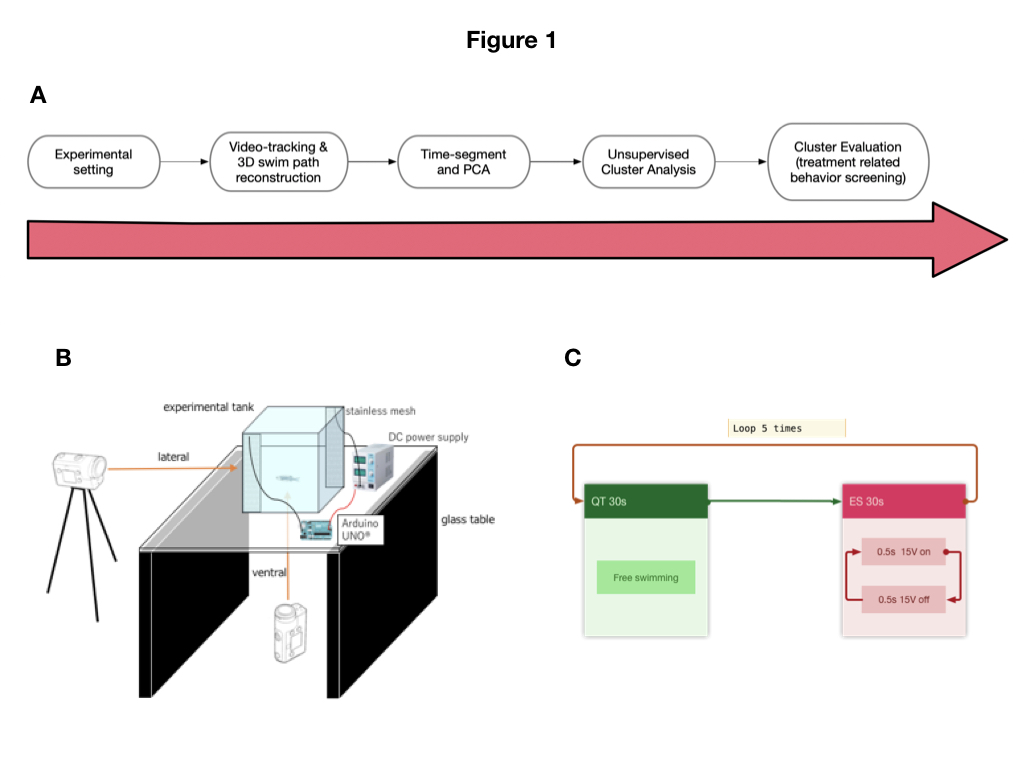
\includegraphics[width=\linewidth]{Figure_1.jpeg}
\caption{Flowchart illustrating the experimental strategy of this study.}
\label{fig:flow}
\end{figure}

\begin{figure}[ht]
\centering
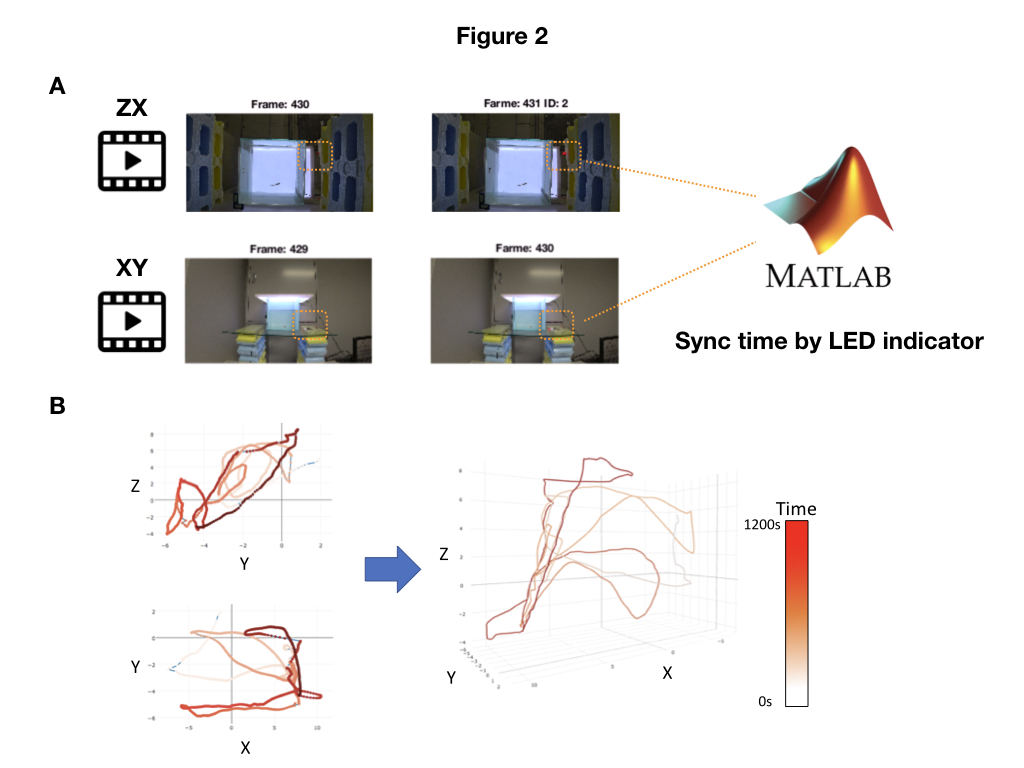
\includegraphics[width=\linewidth]{Figure_2.jpeg}
\caption{Flowchart illustrating the experimental strategy of this study.}
\label{fig:sync}
\end{figure}

\begin{figure}[ht]
\centering
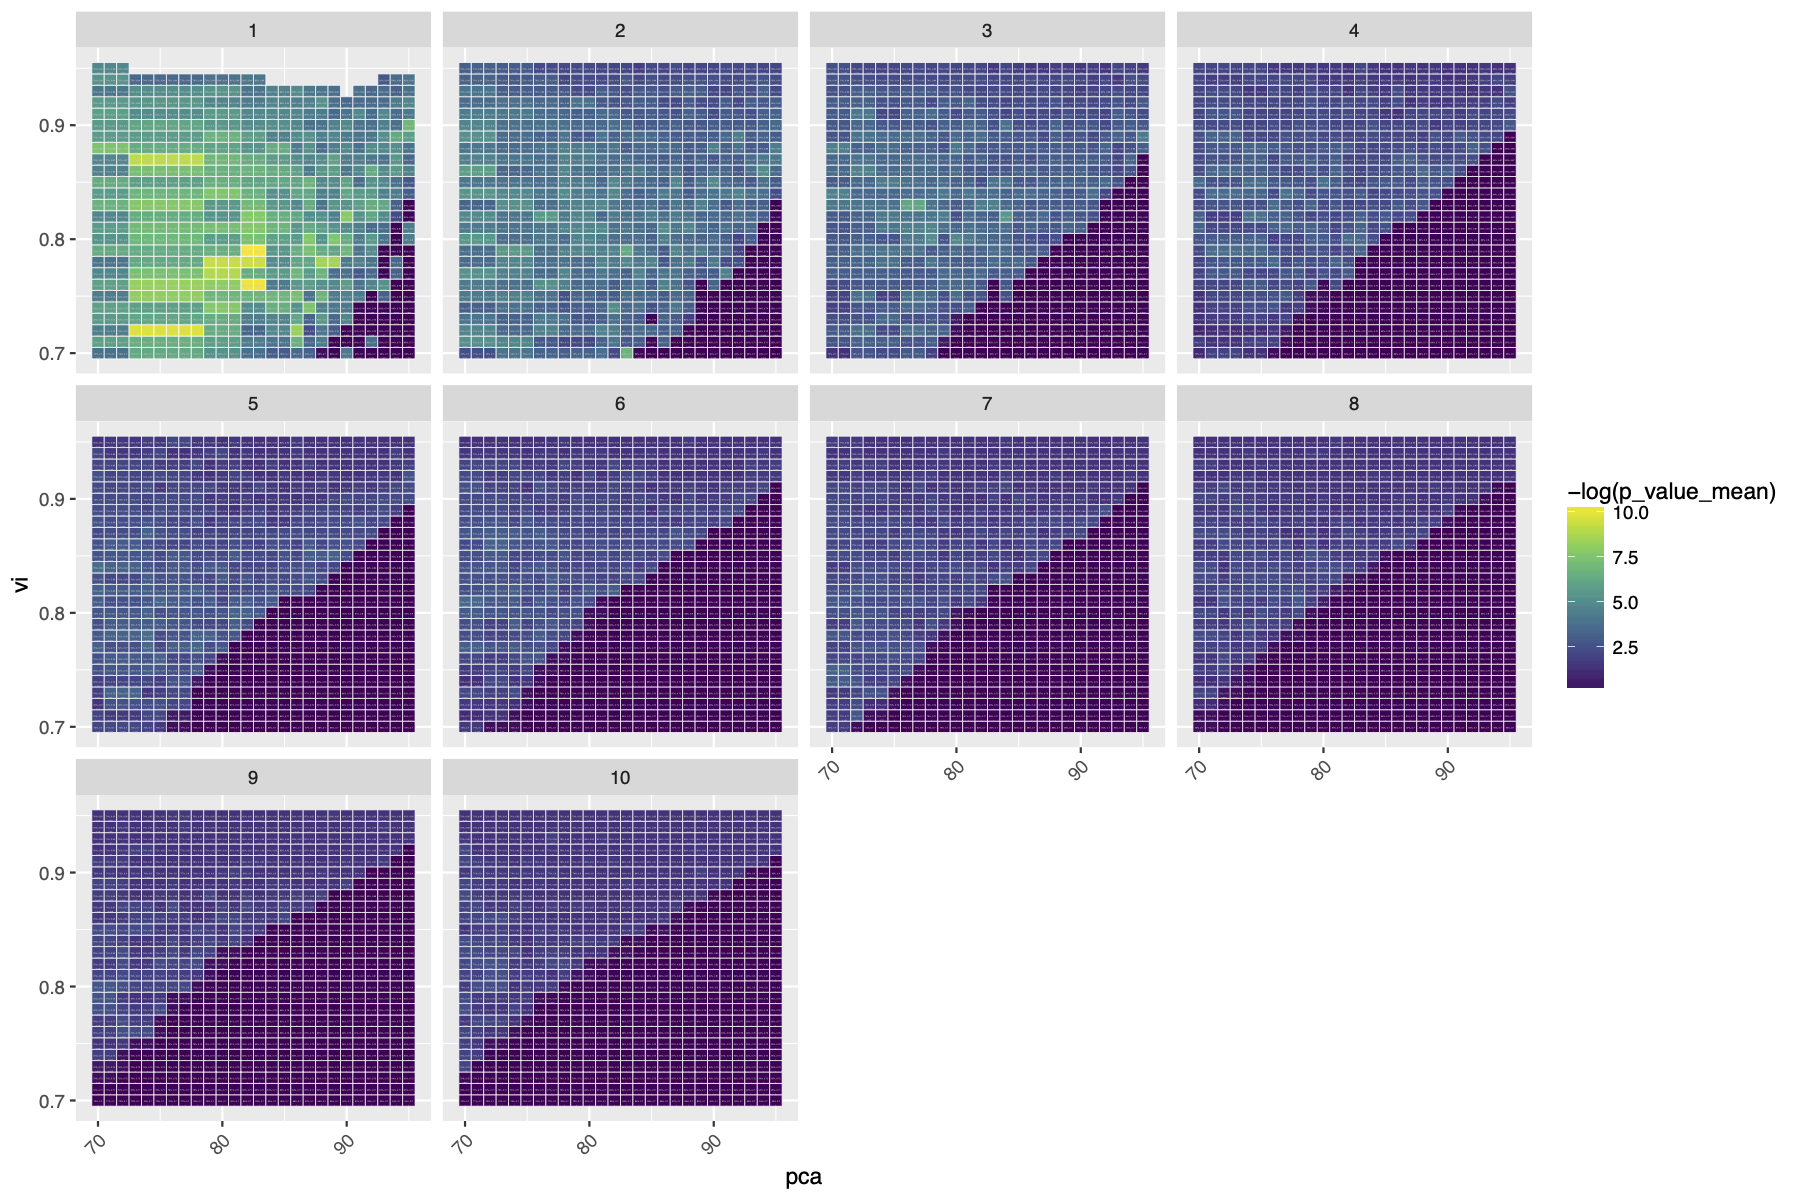
\includegraphics[width=\linewidth]{Figure_3.png}
\caption{Flowchart illustrating the experimental strategy of this study.}
\label{fig:heatmap}
\end{figure}

\begin{figure}[ht]
\centering
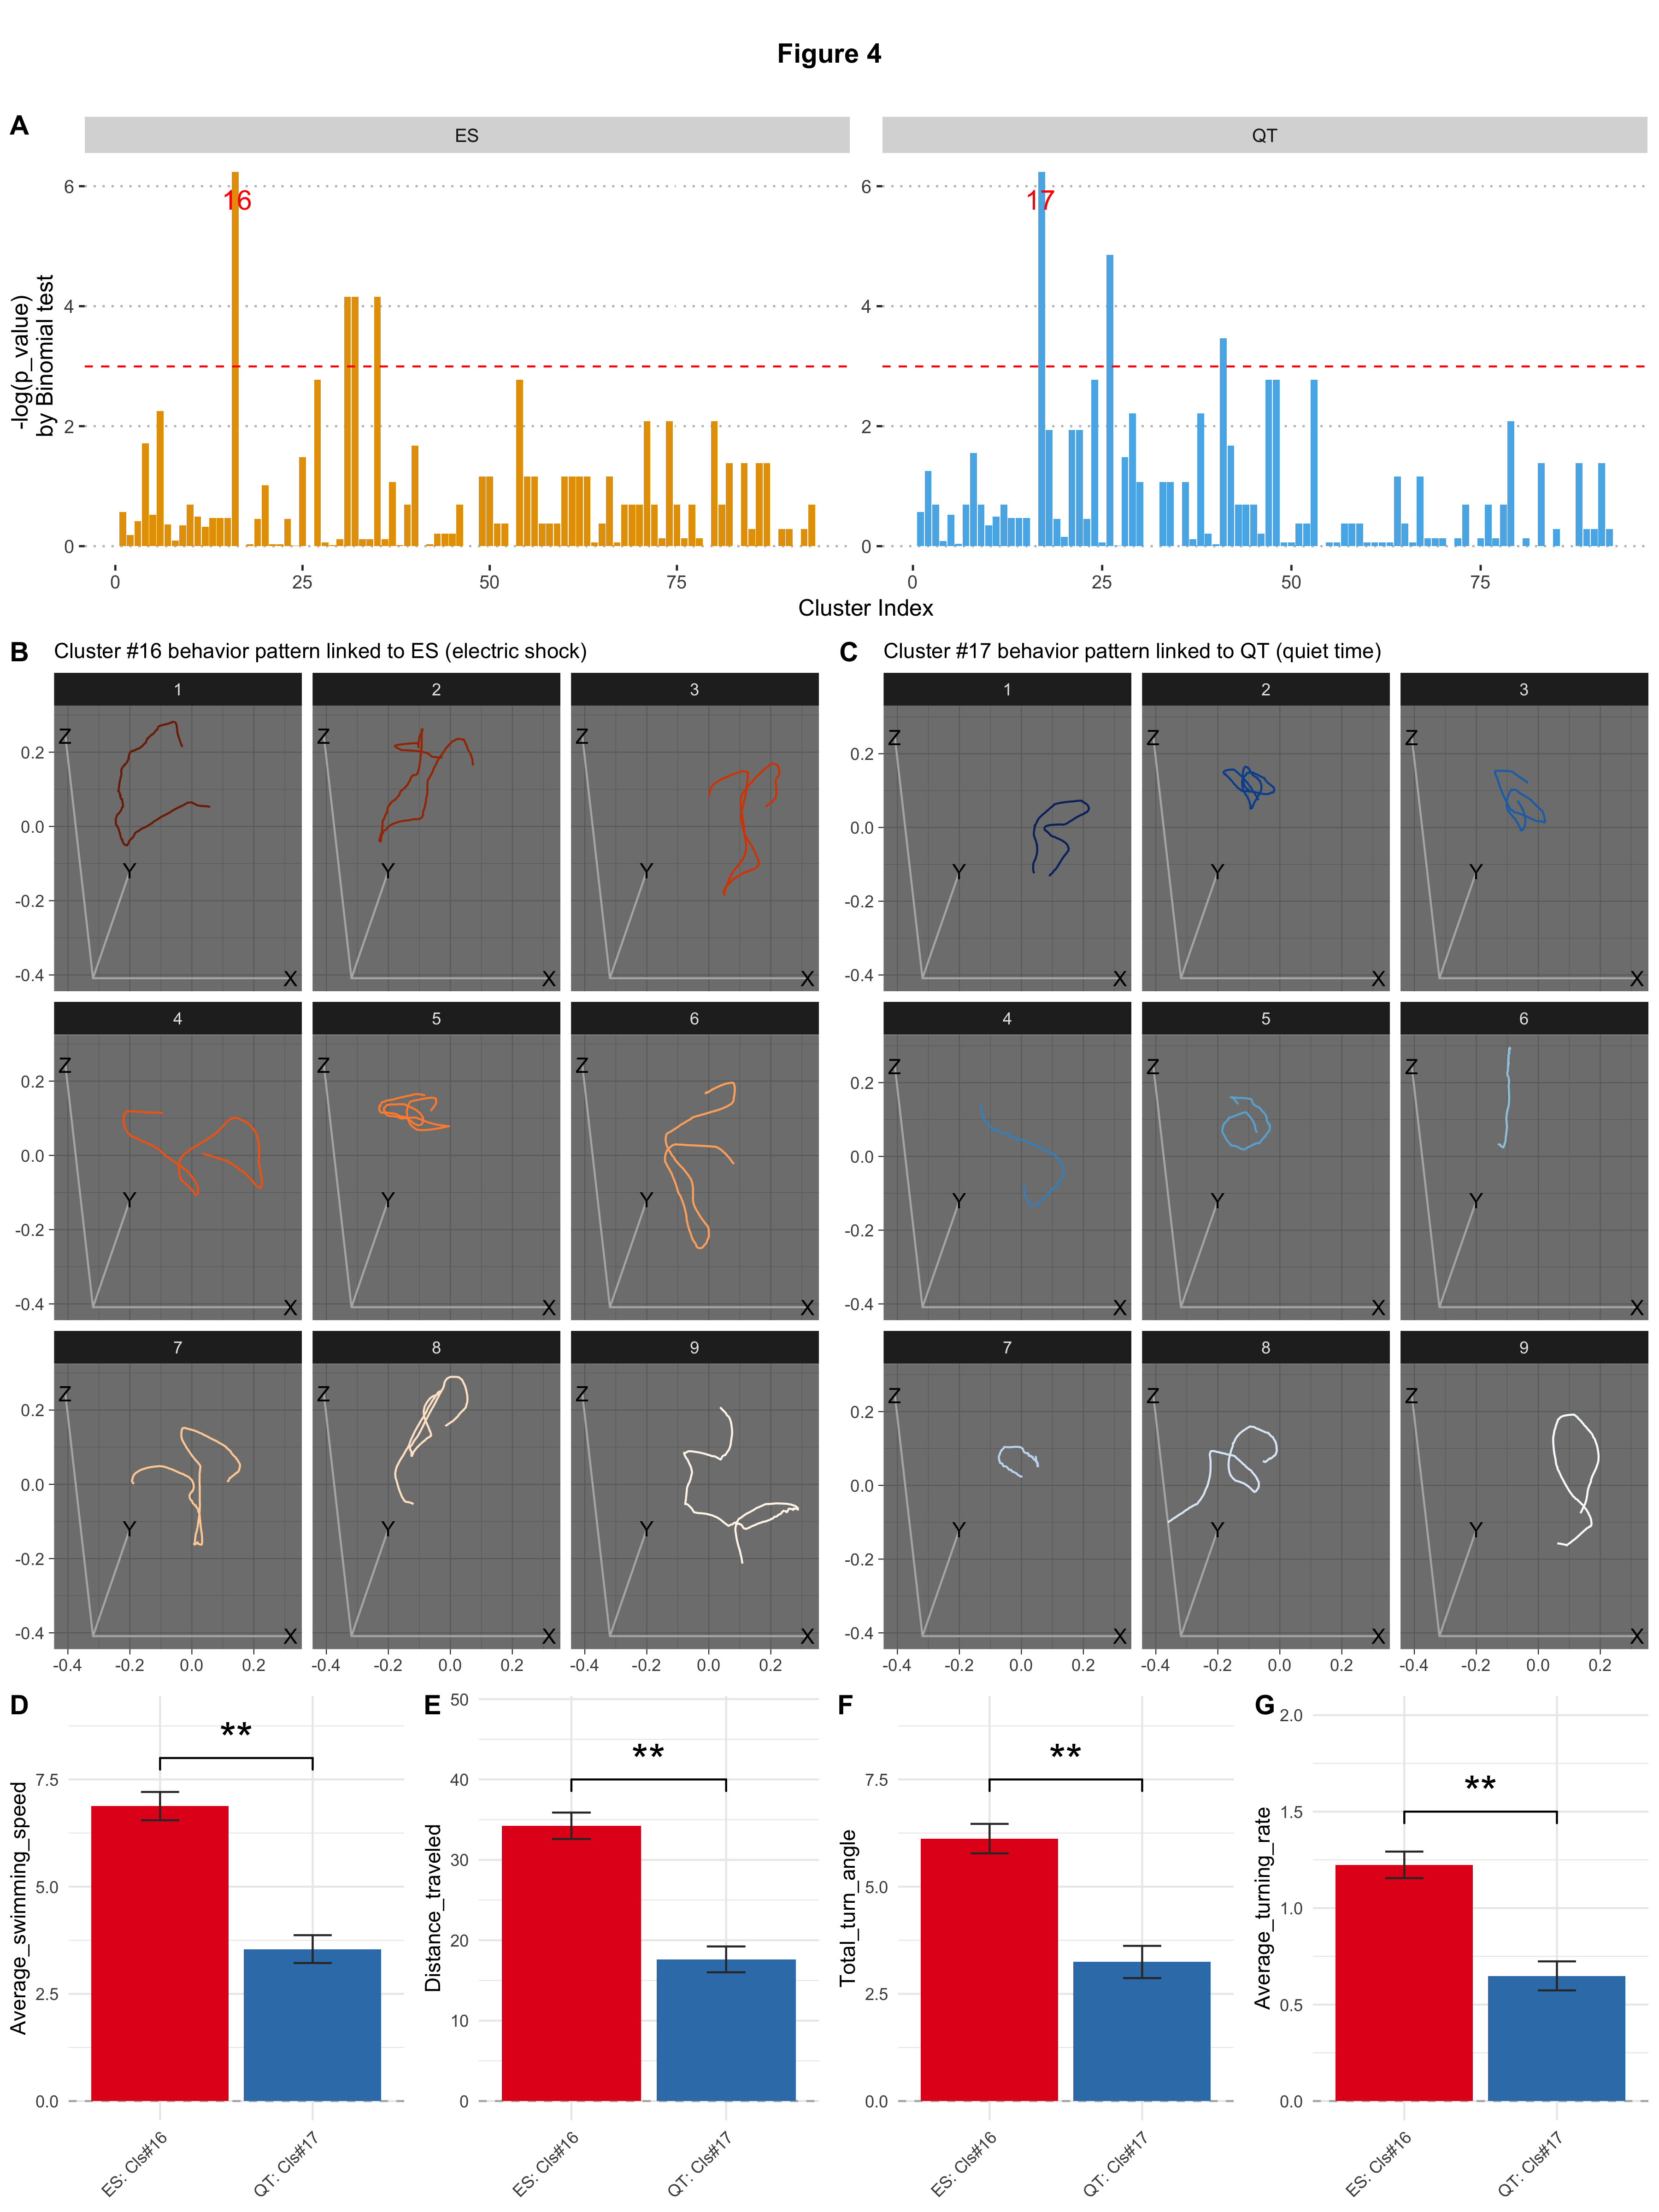
\includegraphics[width=\linewidth]{Figure_4.png}
\caption{Flowchart illustrating the experimental strategy of this study.}
\label{fig:cluster}
\end{figure}

Figures and tables can be referenced in LaTeX using the ref command, e.g. Figure \ref{fig:stream} and Table \ref{tab:example}.

\end{document}